\chapter{Experimentos e Resultados}
\label{chap:ExpRes}
%-------------------------------------------------------------------
Este capítulo contém informações detalhadas sobre os experimentos realizados e os resultados obtidos. Embora o principal caso estudado foi o de degradação dos recursos em virtude de um compartilhamento dos nós, os experimentos realizados podem ser divididos em três categorias de acordo com seu objetivo. As três categorias são: (1) experimentos realizados em ambiente manipulado para verificação do desempenho da solução de forma simplificada; (2) experimentos realizados utilizando a implementação real para verificação do desempenho em ambiente controlado porém próximo à realidade; (3) experimentos em escala para visualização do desempenho com relação à escalabilidade da solução.

\section{Considerações Iniciais Sobre os Experimentos}
Em virtude de algumas informações sobre os experimentos serem comuns à todos eles, como os casos de teste e as aplicações utilizadas, esta Seção é destinada à apresentação destas informações. Além disso, a apresentação dos resultados utiliza diagramas de Gantt com uma estrutura modificada em relação à usualmente encontrada na literatura e será, também, explicada detalhadamente nesta Seção.

\subsection{Casos de teste}
\label{sec:casosteste}
A primeira informação relevante que refere-se à todos experimentos são os casos de teste. Todos os experimentos utilizam os mesmos casos de teste, possuindo apenas objetivos diferentes. Os casos de teste representam situações de compartilhamento, sendo que 2 casos utilizam a implementação padrão e 2 casos utilizam a solução proposta por este trabalho. Além disso, com a criação dos casos de teste buscou-se facilitar a comparação entre os resultados alcançados. A descrição dos casos de testes encontra-se a seguir.

\textbf{Caso \textit{Default} Dedicado (DefDed):} utiliza a versão sem alterações do Hadoop e representa uma situação sem compartilhamento, onde o usuário possui acesso à todos os recursos do \textit{cluster} em qualquer momento. Isto implica que os recursos informados ao escalonador \textbf{sempre} corresponderão aos recursos disponíveis para o Hadoop. Consideram-se recursos informados como os dados que o escalonador utiliza para realizar suas políticas de escalonamento, enquanto, recursos disponíveis são aqueles que estão livres e/ou sendo utilizados pelo próprio Hadoop. Utilizando uma notação percentual, os recursos informados são de 100\% e os recursos disponíveis são de 100\% durante toda execução.

\textbf{Caso \textit{Default} Compartilhado (DefSha):} utiliza a versão sem alterações do Hadoop e representa a situação decorrente do compartilhamento dos nós do \textit{cluster} com outros usuários. Como consequência do compartilhamento, é possível que em, algum momento, ocorra uma inconsistência entre a quantidade de recursos informada e disponível. Este caso aplica o comportamento padrão do Hadoop, no qual os recursos são informados por meio de arquivos XML \textbf{somente} na inicialização do serviço e nunca são atualizados. Para representar a situação onde apenas alguns nós são utilizados, optou-se por deixar alguns nós inalterados e outros com redução de recursos. Nos experimentos de 4 escravos, 2 nós tiveram 6 \textit{cores} e 6 Gb de RAM reduzidos através de um código C, restando 2Gb e 2 \textit{cores} para o SO e Hadoop. No contexto do cluster, os recursos informados são de 100\% enquanto os disponíveis são de 62,5\%.

\textbf{Caso Adaptativo com atualização antes (MyBef):} repete as especificações do Caso DefSha, porém possui a implementação descrita no Capítulo \ref{cap:desen}. Este caso representa a situação de quando o início do compartilhamento ocorre \textbf{antes} da coleta e transmissão de dados, a qual ocorre também \textbf{antes} do lançamento de uma aplicação \textit{MapReduce}. Em ordem cronológica, primeiramente outro usuário inicia a utilização do \textit{cluster}, então a coleta e transmissão de dados ocorre, e finalmente uma aplicação Hadoop é lançada. O resultado desta sequência de eventos é que quando a nova aplicação \textit{MapReduce} for submetida ao \textit{cluster}, este já estará com os dados atualizados. Em notação percentual, os recursos informados são de 62,5\% e os recursos disponíveis são de 62,5\% durante toda aplicação.

\textbf{Caso Adaptativo com atualização durante (MyDur):} representa uma extensão do Caso MyBef (também utilizando a implementação do Capítulo \ref{cap:desen}) na qual o início do compartilhamento ocorre \textbf{antes} da coleta e transmissão dos dados e \textbf{após} a submissão de uma aplicação \textit{MapReduce}. Em ordem cronológica, ocorre o lançamento de uma aplicação \textit{MapReduce}, então quando esta aplicação já está em execução o compartilhamento tem início e finalmente a coleta e transmissão de dados é feita. O resultado desta sequência de eventos é que a aplicação será lançada numa situação onde o \textit{cluster} possui a informação errada (Caso DefSha) e terá de se adaptar à nova configuração dos recursos (Caso MyBef) durante a execução. Em notação percentual, os recursos informados no início da aplicação são de 100\%, enquanto os recursos disponíveis são de 62,5\%. Após a coleta e transmissão de dados os recursos informados também passam a ser 62,5\%.

\subsection{Aplicações de teste}
\label{sec:aplicacoes}
Além dos casos de teste, outra característica importante e comum à todos experimentos são as aplicações. Embora aplicações de \textit{Benchmarks} geralmente possuem dependência de memória, outros fatores como a utilização de CPU e E/S podem influenciar no desempenho. Na busca de indícios de que a solução apresenta ganhos quando utilizada com aplicações de diferentes características, decidiu-se pela utilização de 3 aplicações de \textit{benchmark}, cada uma com diferentes requisições de memória, CPU e E/S. As aplicações são as seguintes:

\begin{itemize}
	\item TeraSort: o objetivo do TeraSort \citep{TeraSort2008} é ordenar um conjunto de dados o mais rápido possível. Este \textit{benchmark} de ordenação estressa tanto a memória como o CPU em virtude das comparações e armazenamento temporário;
	\item WordCount: o \textit{benchmark} WordCount é um exemplo básico de \textit{MapReduce}. Seu objetivo é contar o número de ocorrências de cada palavra de um texto. Como a utilização de memória e E/S é limitada nesta aplicação (tanto a etapa de processamento quanto a saída da aplicação possuem estruturas pequenas em comparação ao arquivo de entrada), o desempenho desta aplicação é determinado pelo CPU;
	\item TestDFSIO: o \textit{benchmark} TestDFSIO é um teste de leitura e escrita para o HDFS. Este \textit{benchmark} é útil para estressar o HDFS, descobrir \textit{bottlenecks} na rede, SO e configuração do Hadoop. O objetivo é prover uma mensuração de quão rápido o \textit{cluster} é em termos de E/S. Tanto a memória quanto o CPU são pouco utilizados.
\end{itemize}

Optou-se pela utilização das aplicações implementadas no \textit{HiBench} \cite{HiBench}, um conjunto de \textit{benchmarks} para \textit{clusters} Hadoop que foi utilizado nos trabalhos \cite{HBA} \cite{HBB} \cite{HBC}. O tamanho de entrada utilizado para cada aplicação nos testes com 4 escravos foi: um conjunto de dados de 15 Gb para o Terasort, 90 arquivos de 250 Mb para o TestDFSIO e um arquivo de 10 Gb para o WordCount. 

\subsection{Configurações de Hardware e Software}
O experimento foi realizado no \textit{cluster} genepi do Grid'5000. A configuração do \textit{cluster} utilizado na maior parte dos experimentos foi a de 1 mestre e 4 escravos, sendo que cada um destes nós possuem a seguinte configuração: 2 CPUs Intel(R) Xeon(R) E5420 2.5GHz (totalizando 8 cores por nó) e 8 Gb RAM. Todos os nós do experimento possuíam o sistema operacional Ubuntu x64-12.04, com a JDK 1.8 instalada e a versão 2.6.0 do Hadoop configurada. Todas as informações foram obtidas através do sistema de \textit{logs} do Hadoop.

\subsection{Apresentação dos resultados}
\label{sec:apresentacao}
Ainda ligado aos experimentos porém com relação aos resultados, os diagramas de Gantt apresentados neste trabalho são modificados para inclusão de mais informações. A apresentação dos diagramas está agrupada por aplicação, sendo que e cada aplicação possui, geralmente, 4 diagramas. Cada um dos diagramas de uma aplicação corresponde a um caso de teste e todos os diagramas de uma aplicação utilizam a mesma escala de tempo.

Cada diagrama possui 2 ou mais linhas, sendo que cada linha representa  um recurso (nó do \textit{cluster}). Estas linhas de recurso possuem diversos separadores verticais (formando diversos segmentos), os quais indicam que ao menos um \textit{container} iniciou/terminou sua execução. Cada segmento apresenta diferentes alturas e tons de cores, os quais são utilizados para representar a carga de \textit{containers Map} do nó. Quanto mais escuro for o tom de um segmento, mais \textit{containers} ele possui em execução; o mesmo aplica-se para a altura do segmento, quanto mais alto mais \textit{containers Map} em execução.

Embora as análises foram feitas principalmente com os \textit{containers} Map, os \textit{containers} de Reduce e do Application Master consomem recursos do \textit{cluster} e devem ser apresentados para uma representação fiel da situação real. Por este motivo, o \textit{container} Application Master é representado na cor azul, os \textit{containers} de Reduce são representados pela cor verde e os \textit{containers} Map são representados em escalas de cinza, sendo branco indicando 0 \textit{containers} e preto indicando o máximo de \textit{containers} em execução em algum momento naquele experimento. Para referência, diagramas da Seção \ref{sec:expCont} possuem máximo de 16, enquanto diagramas das demais Seções possuem máximo de 8.

\section{Experimento controlado}
\label{sec:expCont}
Este experimento foi realizado com objetivo de obter indícios de que a solução poderia contribuir para uma melhora no desempenho do processo de escalonamento quando o Hadoop é utilizado num ambiente onde exista degradação de recursos em virtude de compartilhamento. O experimento simplifica a solução para facilitar a obtenção dos dados em menor tempo. A situação que desejou-se expressar com o experimento é aquela que ocorre quando os nós do \textit{cluster} começam a ser utilizados por outros usuários antes/durante a aplicação \textit{MapReduce}.

\subsection{Procedimentos}
Para que o experimento fosse totalmente controlado, decidiu-se utilizar a manipulação de informações e exclusão de nós para representar o compartilhamento. Na situação real (ver Seção \ref{sec:expReal}) o \textit{cluster} teria 4 escravos e ficaria com uma configuração onde metade dos seus recursos já estariam sendo utilizados por outra aplicação. Por exemplo, outra aplicação utilizaria 4 cores e 4 Gb de memória em cada nó. Para representar esta situação de maneira simples e rápida, o experimento foi realizado com apenas 2 nós (diminuindo os recursos disponíveis pela metade) que tiveram a informação da quantidade de recursos dobrada. Como resultado, o escalonador recebe informação de que os recursos disponíveis são de 16 cores e 16 Gb de memória em cada nó quando na verdade são de apenas 8 cores e 8 Gb. 

Foram realizados experimentos com as 3 aplicações para que as diferenças de comportamento entre elas já pudessem ser estudadas num cenário de sobrecarga de memória e processamento.

\subsection{Resultados e Interpretações}
Os resultados dos experimentos com as aplicações TeraSort, TestDFSIO e WordCount podem ser visualizados nas Tabelas \ref{tab:exp1TS}, \ref{tab:exp1IO} e \ref{tab:exp1WC} e nas Figuras \ref{fig:exp1TS}, \ref{fig:exp1IO} e \ref{fig:exp1WC}, respectivamente.

\begin{table}[h!]
	\caption{Resumo dos resultados do TeraSort controlado em segundos.} \label{tab:exp1TS}
	\begin{tabular*}{\hsize}{lllll} %{\hsize}{@{\extracolsep{\fill}}lllll@{}}
		%\toprule
		\textbf{Caso} & \textbf{DefDed} & \textbf{DefSha} & \textbf{MyBef} & \textbf{MyDur}\\
		\hline
		Tempo Total de Map ({\it{s}}) & 149 & 788 & 348 & 477 \\
		Tempo Médio de Map ({\it{s}}) & 39.47 & 222.97 & 38.38 & 68.42 \\
		%Desvio Padrão & 15.73 & 59.86 & 18.09 & 29.91 \\
		\# Tarefas Map & 76 & 76 & 76 & 76 \\
		\# Tarefas Especulativas & 2 & 1 & 3 & 1 \\
		%\botrule
	\end{tabular*}
\end{table}

\begin{table}[h!]
	\caption{Resumo dos resultados do TestDFSIO controlado em segundos.} \label{tab:exp1IO}
	\begin{tabular*}{\hsize}{lllll} %{\hsize}{@{\extracolsep{\fill}}lllll@{}}
		%\toprule
		\textbf{Caso} & \textbf{DefDed} & \textbf{DefSha} & \textbf{MyBef} & \textbf{MyDur}\\
		\hline
		Tempo Total de Map ({\it{s}}) & 139 & 444 & 239 & 364 \\
		Tempo Médio de Map ({\it{s}}) & 38.95 & 85.01 & 32.20 & 81.62 \\
		%Desvio Padrão & 17.20 & 69.08 & 8.30 & 73.60 \\
		\# Tarefas Map & 90 & 90 & 90 & 90 \\
		\# Tarefas Especulativas & 0 & 9 & 0 & 1 \\
		%\botrule
	\end{tabular*}
\end{table}


\begin{table}[h!]
	\caption{Resumo dos resultados do WordCount controlado em segundos.} \label{tab:exp1WC}
	\begin{tabular*}{\hsize}{lllll} %{\hsize}{@{\extracolsep{\fill}}lllll@{}}
		%\toprule
		\textbf{Caso} & \textbf{DefDed} & \textbf{DefSha} & \textbf{MyBef} & \textbf{MyDur}\\
		\hline
		Tempo Total de Map ({\it{s}}) & 155 & 1009 & 309 & 805 \\
		Tempo Médio de Map ({\it{s}}) & 43.76 & 208.39 & 41.73 & 175.80 \\
		%Desvio Padrão & 15.61 & 128.90 & 10.99 & 151.59 \\
		\# Tarefas Map & 90 & 90 & 90 & 90 \\
		\# Tarefas Especulativas & 1 & 15 & 1 & 10 \\
		%\botrule
	\end{tabular*}
\end{table}

\begin{figure}[!ht]
	\centering
	\includegraphics[height=15cm]{figuras/TeraSort.png}
	\caption{Diagrama de Gantt para os experimentos controlados com TeraSort}
	\label{fig:exp1TS}
\end{figure}

\begin{figure}[!ht]
	\centering
	\includegraphics[height=15cm]{figuras/DFSIO.png}%[width=1\textwidth]
	\caption{Diagrama de Gantt para os experimentos controlados com TestDFSIO}
	\label{fig:exp1IO}
\end{figure}

\begin{figure}[!ht]
	\centering
	\includegraphics[height=15cm]{figuras/WC.png}
	\caption{Diagrama de Gantt para os experimentos controlados com WordCount}
	\label{fig:exp1WC}
\end{figure}

Analisando as tabelas, é possível identificar alguns padrões. Todos experimentos apresentam um comportamento similar com relação ao tempo total dos \textit{containers Map}: DefDed foi o mais rápido, seguido pelos casos MyBef, MyDur e finalmente DefSha. Ainda, os casos DefDed e MyBef possuem os menores tempos médios de \textit{Map} e estes são muito semelhantes não importando a aplicação analizada. Este comportamento é devido à não sobrecarga dos nós, uma vez que o escalonador possuia os dados corretos com relação aos recursos dos nós durante todo experimento.
Os diagramas de Gantt também apresentam esta informação uma vez que os experimentos DefDed e MyBef possuem tons mais claros e alturas menores do que os demais no início da aplicação, o que significa que há menos \textit{containers} em execução. É possível notar também que o caso MyBef leva, em geral, o dobro do tempo do caso DefDed para terminar a etapa de Map. Este resultado é esperado, uma vez que neste experimento o caso DefDed possui o dobro de recursos disponíveis se comparado com o caso MyBef. 

Outra observação interessante tem relação com a análise das tarefas especulativas iniciadas em cada aplicação. A aplicação TeraSort possui um número reduzido de tarefas iniciadas e este número é similar em todos os casos. Já o TestDFSIO e o WordCount apresentam um alto número de tarefas especulativas nos casos em que o sistema está sobrecarregado em algum momento (DefSha e MyDur). Este comportamento pode ser explicado sob a análise dos fatores que determinam o lançamento ou não de uma tarefa especulativa. Sabe-se que uma tarefa especulativa é iniciada com base numa avaliação de progresso da tarefa, onde uma tarefa atrasada em relação às demais está possivelmente apresentando falhas. No caso do TeraSort, onde as tarefas demandam de maneira uniforme os recursos de memória, CPU e E/S, o tempo de execução está menos sujeito à redução de um recurso específico. Enquanto o TestDFSIO e o WordCount, demandam recursos mais específicos e, portanto, são mais sensíveis à sobrecarga destes recursos. Em todas as aplicações, a utilização de sensibilidade ao contexto como meio de melhorar a adaptabilidade no caso MyDur ajuda a reduzir o número de tarefas especulativas quando comparado com o caso DefSha que não apresenta nenhuma capacidade de adaptação à estes ambientes.

Com relação ao fluxo de execução, como ilustrado nos diagramas, é possível notar que os casos DefSha e MyDur possuem tons mais escuros no início, o que significa que cada nó está com 16 \textit{containers} em execução (o dobro da capacidade real do nó). Ainda, os primeiros \textit{containers} a terminar nos casos DefDed e MyBef levam entre 20 e 50 segundos (conforme linha vertical de segmento), enquanto nos casos DefSha (e em menor grau MyDur) os primeiros \textit{containers} levam 70 segundos ou mais para terminar, evidenciando a sobrecarga dos nós. As excessões à esta afirmação são os casos DefSha e MyDur do TestDFSIO, nos quais os primeiros \textit{containers} a terem o processamento concluído levam aproximadamente 25 segundos para tal. Através de uma análise mais profunda, é possível notar que todos os casos do experimento TestDFSIO possuem ao menos um seguimento próximo à marca dos 25 segundos, o que significa que uma das tarefas deste conjunto de entrada foi processada rapidamente em todos os casos, e não foi afetada pela sobrecarga dos nós nos casos DefSha e MyDur.

Embora os casos DefSha e MyDur possuam as mesmas condições iniciais (recursos disponíveis de 50\% e recursos informados de 100\%), o caso MyDur necessita de menos tempo para concluir o processamento da aplicação em todas as aplicações. O caso MyDur possui uma melhora de 20\% a 40\% no tempo de execução quando comparado com o caso DefSha. A razão para este comportamento é a capacidade de adaptação inserida ao Hadoop, a qual permite que os Node Managers coletem a informação correta e à transmitam para o escalonador, que irá reorganizar a distribuição de tarefas à medida que as tarefas em execução são concluídas. Este comportamento é mais fácil de ser observado nos diagramas das aplicações TeraSort e TestDFSIO. É possível notar também que todos o casos MyDur possuem alta concentração de containers no início da aplicação mas essa concentração diminui ao longo da execução, enquanto os casos DefSha mantém a alta concentração até os últimos momentos da execução devido à ausencia de adaptabilidade. Embora o escalonador não preempte \textit{containers} em excesso, é possível observar uma melhora de aproximadamente 40\% no TeraSort e 20\% no TestDFSIO e WordCount apenas pela inibição do lançamento de novos \textit{containers} enquanto o nó está sobrecarregado.


%Although other specificities about the characteris-
%tics of the proposed jobs can be discussed, scenarios C
%and D show that regular context updates contribute to
%reduce the execution time on a dynamic Hadoop clus-
%ter. We demonstrated that even when starting with the
%same circumstances of the worst case (Scenario B), up-
%dating the information helps the scheduler to minimize
%the execution time. Our solution contributes therefore
%to both provide correct information before the execu-
%tion starts (Scenario C) and to adapt the execution to
%resources changes (Scenario D).
%CONCLUSÂO

\section{Experimento real}
\label{sec:expReal}
Este experimento foi realizado com objetivo de obter indícios de que a solução poderia contribuir para uma melhora no desempenho do processo de escalonamento quando o Hadoop é utilizado num ambiente onde exista degradação de recursos em virtude de compartilhamento. O experimento utiliza a solução descrita no Capítulo \ref{cap:desen}. A situação expressada com este experimento é de quando os nós do \textit{cluster} começam a ser utilizados por outros usuários antes/durante a aplicação \textit{MapReduce}.

\subsection{Procedimentos}
Diferentemente do experimento anterior, neste experimento buscou-se o comportamento da solução em um ambiente realmente compartilhado. O \textit{cluster} possui 4 escravos e alguns escravos terão, em algum momento, seus recursos disponíveis reduzidos devido ao compartilhamento, ou seja, outra aplicação irá utilizar 6 cores e 6 Gb de memória em 2 dos 4 nós escravos. Para alcançar esta situação foi implementada uma aplicação em C, na qual a quantidade desejada de \textit{threads} é inicializada e cada uma delas utiliza 1 core e 1 Gb de memória. O experimento foi realizado com as 3 aplicações para observações de possíveis alterações no comportamento com relação ao experimento inicial.

\subsection{Resultados e Interpretações}
Os resultados dos experimentos com as aplicações TeraSort, TestDFSIO e WordCount podem ser visualizados nas Tabelas \ref{tab:exp2TS}, \ref{tab:exp2IO} e \ref{tab:exp2WC} e nas Figuras \ref{fig:exp2TS}, \ref{fig:exp2IO} e \ref{fig:exp2WC}, respectivamente.

\begin{table}[h!]
	\caption{Resumo dos resultados do TeraSort real em segundos.} \label{tab:exp2TS}
	\begin{tabular*}{\hsize}{lllll} %{\hsize}{@{\extracolsep{\fill}}lllll@{}}
		%\toprule
		\textbf{Caso} & \textbf{DefDed} & \textbf{DefSha} & \textbf{MyBef} & \textbf{MyDur}\\
		\hline
		Tempo Total de Map ({\it{s}}) & 281 & 1372 & 740 & 888 \\
		Tempo Médio de Map ({\it{s}}) & 38.50 & 198.86 & 39.58 & 62.82 \\
		%Desvio Padrão & 15.73 & 59.86 & 18.09 & 29.91 \\
		\# Tarefas Map & 112 & 112 & 112 & 112 \\
		\# Tarefas Especulativas & 1 & 14 & 0 & 2 \\
		%\botrule
	\end{tabular*}
\end{table}

\begin{table}[h!]
	\caption{Resumo dos resultados do TestDFSIO real em segundos.} \label{tab:exp2IO}
	\begin{tabular*}{\hsize}{lllll} %{\hsize}{@{\extracolsep{\fill}}lllll@{}}
		%\toprule
		\textbf{Caso} & \textbf{DefDed} & \textbf{DefSha} & \textbf{MyBef} & \textbf{MyDur}\\
		\hline
		Tempo Total de Map ({\it{s}}) & 194 & 674 & 264 & 431 \\
		Tempo Médio de Map ({\it{s}}) & 31.24 & 162.47 & 38.56 &  65.24 \\
		%Desvio Padrão & 17.20 & 69.08 & 8.30 & 73.60 \\
		\# Tarefas Map & 90 & 90 & 90 & 90 \\
		\# Tarefas Especulativas & 2 & 16 & 0 & 8 \\
		%\botrule
	\end{tabular*}
\end{table}


\begin{table}[h!]
	\caption{Resumo dos resultados do WordCount real em segundos.} \label{tab:exp2WC}
	\begin{tabular*}{\hsize}{lllll} %{\hsize}{@{\extracolsep{\fill}}lllll@{}}
		%\toprule
		\textbf{Caso} & \textbf{DefDed} & \textbf{DefSha} & \textbf{MyBef} & \textbf{MyDur}\\
		\hline
		Tempo Total de Map ({\it{s}}) & 153 & 533 & 361 & 396 \\
		Tempo Médio de Map ({\it{s}}) & 34.85 & 105.27 & 37.79 & 57.76 \\
		%Desvio Padrão & 15.61 & 128.90 & 10.99 & 151.59 \\
		\# Tarefas Map & 90 & 90 & 90 & 90 \\
		\# Tarefas Especulativas & 1 & 14 & 1 & 2 \\
		%\botrule
	\end{tabular*}
\end{table}

\begin{figure}[!ht]
	\centering
	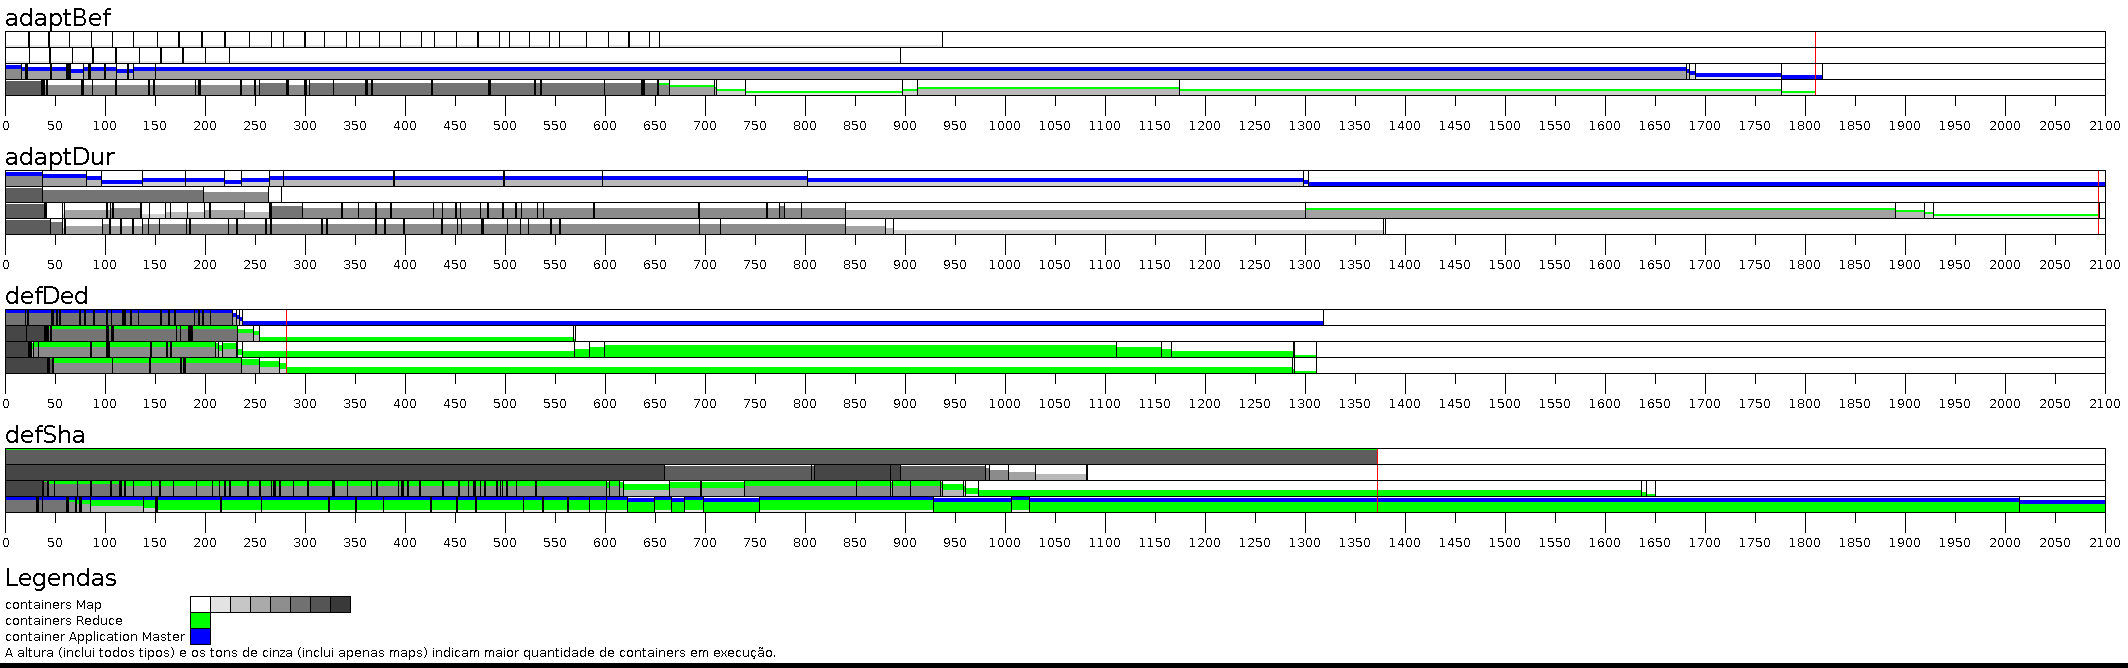
\includegraphics[width=1\textwidth]{figuras/TS-real.png}
	\caption{Diagrama de Gantt para os experimentos reais com TeraSort}
	\label{fig:exp2TS}
\end{figure}

\begin{figure}[!ht]
	\centering
	\includegraphics[height=15cm]{figuras/DFSIO-real.png}
	\caption{Diagrama de Gantt para os experimentos reais com TestDFSIO}
	\label{fig:exp2IO}
\end{figure}

\begin{figure}[!ht]
	\centering
	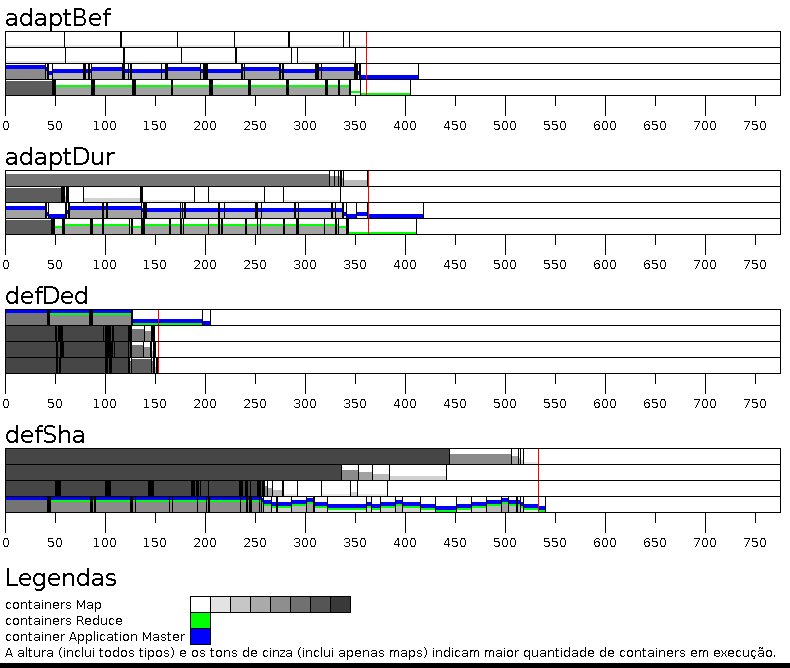
\includegraphics[height=15cm]{figuras/WC-real.png}
	\caption{Diagrama de Gantt para os experimentos reais com WordCount}
	\label{fig:exp2WC}
\end{figure}

Através da análise das tabelas e dos diagramas, nota-se que muitos padrões foram mantidos apesar da alteração de procedimento nos experimentos. Primeiramente, é importante notar que nas aplicações anteriores a sobrecarga dos nós era de 100\%, uma vez que o Hadoop estava tentando utilizar o dobro da capacidade. Na execução das aplicações deste experimento a sobrecarga é levemente menor, pois a informação passada ao Hadoop nos casos default não é alterada. A sobrecarga nestes experimentos é de aproximadamente 6 Gb de RAM e 6 cores, fazendo com que o nó, nos piores casos, tenha uma demanda de aproximadamente 14 Gb e 14 cores (sem considerar recursos requisitados pelo sistema operacional e serviços do Hadoop) alocada aos seus 8 Gb e 8 cores.

Novamente, todas aplicações apresentam um comportamento similar com relação ao tempo total dos \textit{containers Map} e tempo médio destes: DefDed apresentou o menor tempo total e médio dos \textit{containers Map}, seguido pelos casos MyBef, MyDur e finalmente DefSha. Também seguindo o padrão do experimento anterior, os tempos médio de Map nos casos DefDed e MyBef são muito semelhantes não importando a aplicação analizada. Embora alguns padrões foram mantidos, a proporção de tempo entre os casos DefDed e MyBef não apresenta uma relação tão constante quanto no experimento anterior e algumas particularidades podem ser observadas nos diagramas. Ainda assim, estes dados iniciais sugerem que uma sobrecarga de alguns nós, mesmo em menor intensidade se comparado ao experimento anterior, deteriora significativamente o desempenho da aplicação.

Com relação às tarefas especulativas, nota-se que neste experimento o caso DefSha apresentou um número alto de tarefas especulativas nas 3 aplicações, enquanto os demais casos mantiveram valores baixos salvo o caso MyDur na aplicação TestDFSIO. Os resultados deste experimento sugerem que embora a sobrecarga, com relação à demanda total, tenha sido menor, os efeitos provocados por ela foram mais visíveis, pois os casos onde a sobrecarga esteve presente durante toda aplicação apresentam um número elevado de tarefas especulativas.

Antes de realizar a análise dos diagramas deste experimento é necessário salientar uma característica importante, todos os diagramas a gerados para este experimento possuem no máximo 8 \textit{containers} em execução, enquanto no experimento anterior este valor era de 16. Além disso, os diagramas possuem características que permitem uma visualização das tarefas que originam tarefas especulativas e da reação à mudança de recursos nos nós. 

Nas 3 aplicações o caso MyBef pode, em um primeiro momento, aparentar estar com 2 nós sem utilização, porém este comportamento é exatamente o esperado dos nós. O caso de teste é criado de forma que quando outro usuário utiliza o \textit{cluster}, ele demanda 6 Gb e 6 cores de 50\% dos nós, deixando apenas 2 Gb e 2 cores disponíveis para o sistema operacional e o Hadoop. Retirando os recursos do sistema operacional e dos serviços do Hadoop restam pouco mais de 1 Gb e 1 core livres, com os quais o Hadoop pode lançar apenas 1 \textit{container} nos nós compartilhados. Com apenas 1 \textit{container} em execução, o diagrama apresenta uma cor próxima do branco e a altura de somente 1/8 da linha, tornando a visualização de \textit{containers} Map difícil. No caso de um \textit{container} Reduce em execução, como no diagrama MyBef do TestDFSIO, a cor verde facilita a visualização.

Nos diagramas gerados para os casos MyDur da aplicação TestDFSIO é possível notar que um dos nós termina uma carga de 6 a 7 containers simultaneamente e que logo após isso a aplicação toda é concluída. Uma rápida consulta à tabela fornece a informação de que nessa aplicação o número de tarefas especulativas no caso MyDur foi o mais elevado das 3 aplicações. Além disso, a análise dos logs mostra que a última tarefa especulativa termina 2 segundos antes do término de todos \textit{containers} do primeiro nó. Estas duas observações sugerem que a sobrecarga do nó compartilhado impediu o término gradual dos \textit{containers} lentos à medida que suas cópias especulativas finalizavam a execução. Este mesmo comportamento pode ser observado no caso DefSha.

Apesar das condições e mecanismos de compartilhamento/atualização implementados nos testes reais serem diferentes daqueles implementados nos testes controlados, os diagramas deste experimento também apresentam reação ao início do compartilhamento. É possível notar uma redução gradual dos recursos nos dois primeiros nós na maioria dos casos MyDur. Além disso, é possível notar que a linha nunca fica completamente colorida nos casos MyBef e MyDur, indicando que o coletor detectou os recursos utilizados pelo sistema operacional e excluiu os mesmos do \textit{pool} de recursos do Hadoop.

Mais uma vez as execuções do caso MyDur apresentam uma melhora entre 36\% e 24\% no tempo total de Map comparado com o caso DefSha, mostrando que a detecção da sobrecarga no nó e a adaptação do processo de escalonamento para eventualmente eliminar a sobrecarga melhora o desempenho da aplicação. Ainda com relação ao tempo total de Map, nota-se que quanto maior a duração da aplicação maior é o ganho de desempenho pela utilização do escalonamento adaptativo. Os resultados também indicam que a adaptação do escalonamento em função da sobrecarga diminui a quantidade de tarefas especulativas e o tempo médio que as tarefas Map levam para concluir a execução. 


\section{Experimento de escala}
Uma vez que os experimentos anteriores já responderam algumas questões importantes sobre a viabilidade da solução implementada, este experimento foi realizado com objetivo de analisar se as melhorias no escalonamento são mantidas quando o Hadoop é utilizado em um ambiente ou com uma entrada de dados maior. O experimento utiliza a solução descrita no Capítulo \ref{cap:desen}. A situação expressada com este experimento é de quando os nós do \textit{cluster} começam a ser utilizados por outros usuários antes/durante a aplicação \textit{MapReduce}.

\subsection{Procedimentos}
Neste experimento buscou-se analisar o comportamento da solução em um ambiente compartilhado de maior escala que nos experimentos anteriores. Foram feitos 2 experimentos distintos, um com escala de aplicação outro com escala de ambiente. Para a escala de aplicação a única diferença das configurações foi o tamanho da entrada, sendo utilizada uma entrada de 32 Gb para o TeraSort. Para a escala de ambiente, utilizou-se um \textit{cluster} com X escravos, sendo que a proporção de recursos reduzidos/livres continuou a mesma. 

\subsection{Resultados e Interpretações}
Os resultados dos experimentos em escala (de entrada e de ambiente) com a aplicação TeraSort podem ser visualizados nas Tabelas \ref{tab:exp3TS} e \ref{tab:exp31TS} e nas Figuras \ref{fig:exp3TS} e \ref{fig:exp31TS}, respectivamente.

\begin{table}[h!]
	\caption{Resumo dos resultados do TeraSort em escala (tamanho da entrada) em segundos.} \label{tab:exp3TS}
	\begin{tabular*}{\hsize}{l|llll} %{\hsize}{@{\extracolsep{\fill}}lllll@{}}
		%\toprule
		\textbf{Caso} & \textbf{DefDed} & \textbf{DefSha} & \textbf{MyBef} & \textbf{MyDur}\\
		\hline
		Tempo Total de Map ({\it{s}}) & 1357 & 4627 & 2060 & 2184 \\
		Tempo Médio de Map ({\it{s}}) & 43.39 & 299.70 & 45.36 & 65.00 \\
		\# Tarefas Map & 240 & 240 & 240 & 240 \\
		\# Tarefas Especulativas & 1 & 27 & 0 & 5 \\
		%\botrule
	\end{tabular*}
\end{table}
%
%


\begin{table}[h!]
	\caption{Resumo dos resultados do TeraSort em escala (tamanho do ambiente) em segundos.} \label{tab:exp31TS}
	\begin{tabular*}{\hsize}{l|llll} %{\hsize}{@{\extracolsep{\fill}}lllll@{}}
		%\toprule
		\textbf{Caso} & \textbf{DefDed} & \textbf{DefSha} & \textbf{MyBef} & \textbf{MyDur}\\
		\hline
		Tempo Total de Map ({\it{s}}) & 1357 & 4627 & 2060 & 2184 \\
		Tempo Médio de Map ({\it{s}}) & 43.39 & 299.70 & 45.36 & 65.00 \\
		\# Tarefas Map & 240 & 240 & 240 & 240 \\
		\# Tarefas Especulativas & 1 & 27 & 0 & 5 \\
		%\botrule
	\end{tabular*}
\end{table}
%
%

\begin{sidewaysfigure}
    \centering
	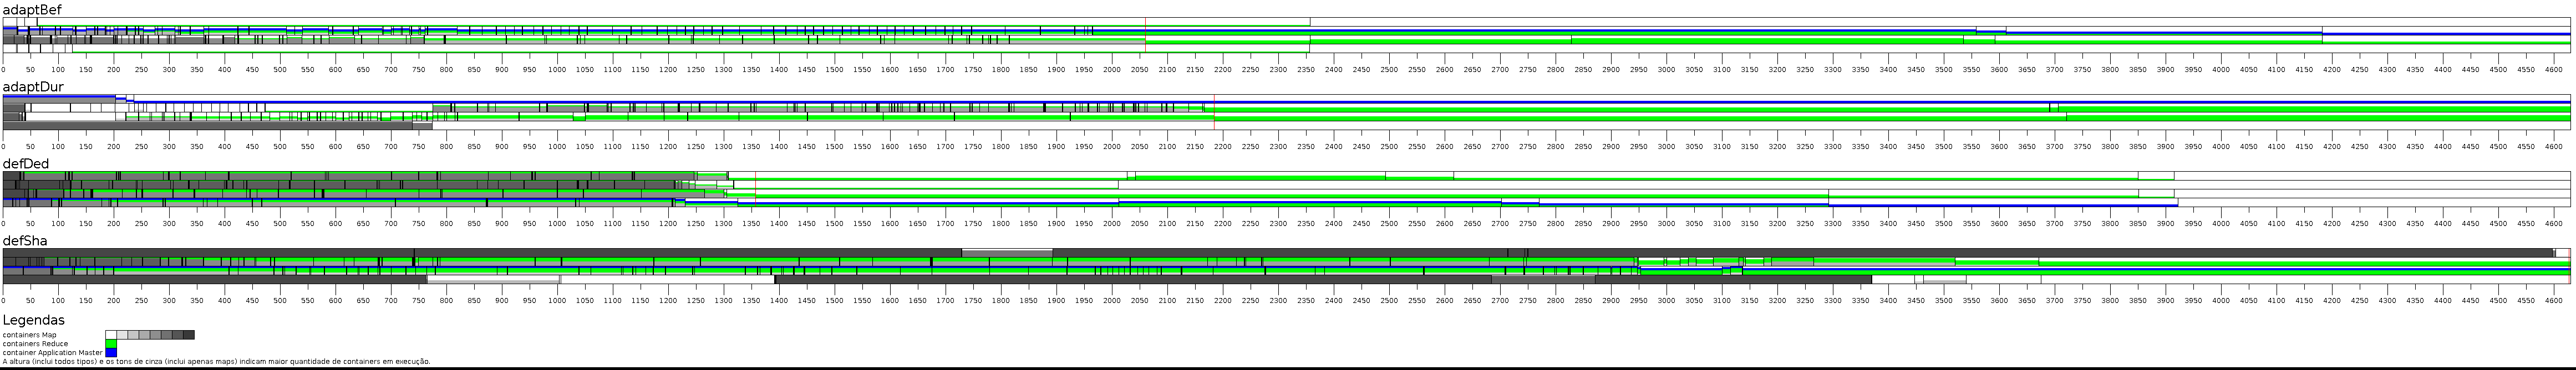
\includegraphics[width=1\textwidth]{figuras/TS-esc-ent.png}
    \caption{Diagrama de Gantt para o experimento em escala (tamanho da entrada) com TeraSort}
	\label{fig:exp3TS}

	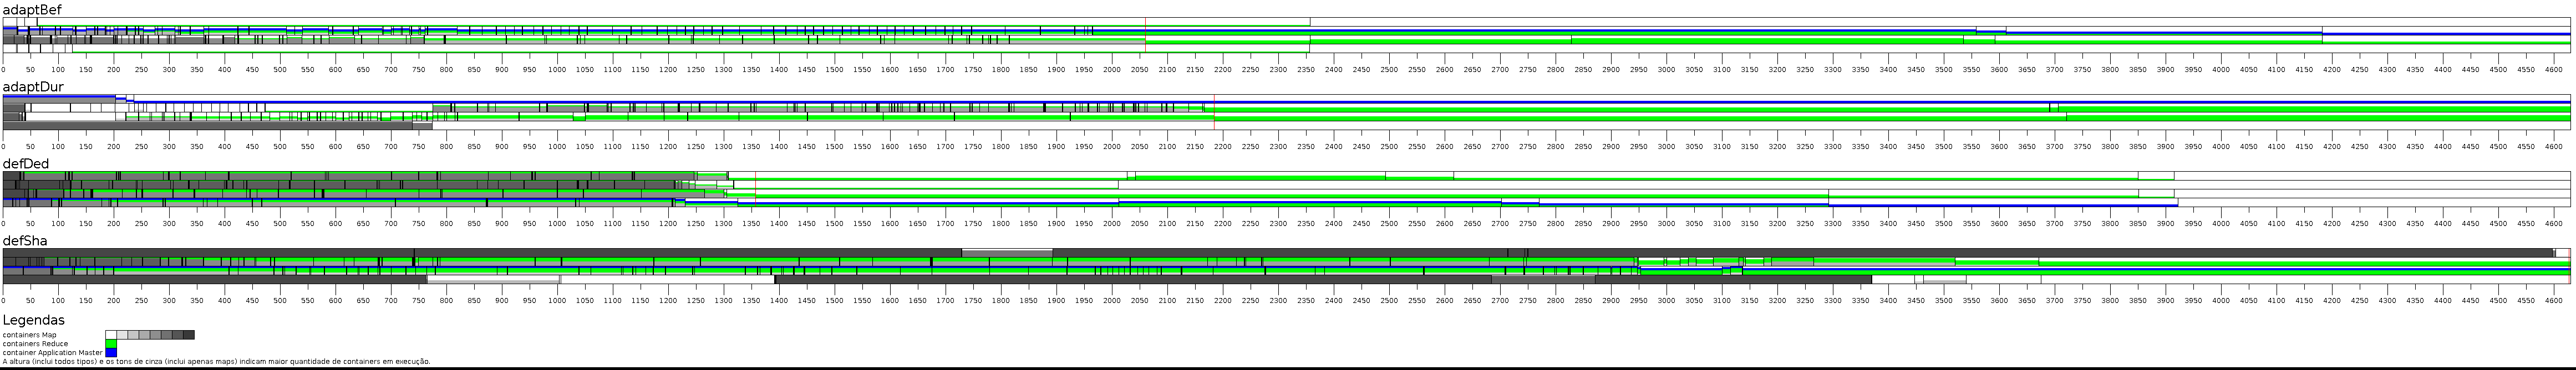
\includegraphics[width=1\textwidth]{figuras/TS-esc-ent.png}
    \caption{Diagrama de Gantt para o experimento em escala (tamanho do ambiente) com TeraSort}
	\label{fig:exp31TS}	
\end{sidewaysfigure}



No experimento realizado com o tamanho da entrada maior pode-se notar que o caso MyBef apresentou um tempo de execução mais rápido que o experado. O tempo de execução atingido foi aproximadamente 50\% maior comparado com o caso DefDed, porém o esperado era de 100\%. Este valor era esperado pois no caso MyBef a configuração dos recursos alocáveis é de 2 escravos com 1Gb/core e 2 escravos com 7Gb/cores enquanto a configuração dos recursos alocáveis no caso DefDed é de 4 escravos com 8Gb/cores. Este resultado sugere que desconsiderar os recursos utilizados pelo sistema operacional e serviços do Hadoop já cria uma sobrecarga no nó, porém esta só é facilmente perceptível em aplicações que possuem um tempo de execução mais elevado. Este mesmo motivo pode ser a causa do caso MyBef não apresentar tarefas especulativas, enquanto o caso DefDed apresenta 1.

Nota-se, mais uma vez, que os tempos de execução das aplicações apresenta a ordem DefDed, MyBef, MyDur e DefSha. Contudo, neste experimento a diferença de tempo entre os casos DefDed e MyBef, tanto do tempo total como do tempo médio dos \textit{containers} é maior, sugerindo que a solução deste trabalho possui uma efetividade diretamente proporcional ao tamanho da aplicação que é executada.

HAHAHA


%
%Analisando as tabelas, é possível identificar alguns padrões. Todos experimentos apresentam um comportamento similar com relação ao tempo total dos \textit{containers Map}: DefDed foi o mais rápido, seguido pelos casos MyBef, MyDur e finalmente DefSha. Ainda, os casos DefDed e MyBef possuem os menores tempos médios de \textit{Map} e estes são muito semelhantes não importando a aplicação analizada. Este comportamento é devido à não sobrecarga dos nós, uma vez que o escalonador possuia os dados corretos com relação aos recursos dos nós durante todo experimento.
%Os diagramas de Gantt também apresentam esta informação uma vez que os experimentos DefDed e MyBef possuem tons mais claros e alturas menores do que os demais no início da aplicação, o que significa que há menos \textit{containers} em execução. É possível notar também que o caso MyBef leva, em geral, o dobro do tempo do caso DefDed para terminar a etapa de Map. Este resultado é esperado, uma vez que neste experimento o caso DefDed possui o dobro de recursos disponíveis se comparado com o caso MyBef. 
%
%Outra observação interessante tem relação com a análise das tarefas especulativas iniciadas em cada aplicação. A aplicação TeraSort possui um número reduzido de tarefas iniciadas e este número é similar em todos os casos. Já o TestDFSIO e o WordCount apresentam um alto número de tarefas especulativas nos casos em que o sistema está sobrecarregado em algum momento (DefSha e MyDur). Este comportamento pode ser explicado sob a análise dos fatores que determinam o lançamento ou não de uma tarefa especulativa. Sabe-se que uma tarefa especulativa é iniciada com base numa avaliação de progresso da tarefa, onde uma tarefa atrasada em relação às demais está possivelmente apresentando falhas. No caso do TeraSort, onde as tarefas demandam de maneira uniforme os recursos de memória, CPU e E/S, o tempo de execução está menos sujeito à redução de um recurso específico. Enquanto o TestDFSIO e o WordCount, demandam recursos mais específicos e, portanto, são mais sensíveis à sobrecarga destes recursos. Em todas as aplicações, a utilização de sensibilidade ao contexto como meio de melhorar a adaptabilidade no caso MyDur ajuda a reduzir o número de tarefas especulativas quando comparado com o caso DefSha que não apresenta nenhuma capacidade de adaptação à estes ambientes.
%
%Com relação ao fluxo de execução, como ilustrado nos diagramas, é possível notar que os casos DefSha e MyDur possuem tons mais escuros no início, o que significa que cada nó está com 16 \textit{containers} em execução (o dobro da capacidade real do nó). Ainda, os primeiros \textit{containers} a terminar nos casos DefDed e MyBef levam entre 20 e 50 segundos (conforme linha vertical de segmento), enquanto nos casos DefSha (e em menor grau MyDur) os primeiros \textit{containers} levam 70 segundos ou mais para terminar, evidenciando a sobrecarga dos nós. As excessões à esta afirmação são os casos DefSha e MyDur do TestDFSIO, nos quais os primeiros \textit{containers} a terem o processamento concluído levam aproximadamente 25 segundos para tal. Através de uma análise mais profunda, é possível notar que todos os casos do experimento TestDFSIO possuem ao menos um seguimento próximo à marca dos 25 segundos, o que significa que uma das tarefas deste conjunto de entrada foi processada rapidamente em todos os casos, e não foi afetada pela sobrecarga dos nós nos casos DefSha e MyDur.
%
%Embora os casos DefSha e MyDur possuam as mesmas condições iniciais (recursos disponíveis de 50\% e recursos informados de 100\%), o caso MyDur necessita de menos tempo para concluir o processamento da aplicação em todas as aplicações. O caso MyDur possui uma melhora de 20\% a 40\% no tempo de execução quando comparado com o caso DefSha. A razão para este comportamento é a capacidade de adaptação inserida ao Hadoop, a qual permite que os Node Managers coletem a informação correta e à transmitam para o escalonador, que irá reorganizar a distribuição de tarefas à medida que as tarefas em execução são concluídas. Este comportamento é mais fácil de ser observado nos diagramas das aplicações TeraSort e TestDFSIO. É possível notar também que todos o casos MyDur possuem alta concentração de containers no início da aplicação mas essa concentração diminui ao longo da execução, enquanto os casos DefSha mantém a alta concentração até os últimos momentos da execução devido à ausencia de adaptabilidade. Embora o escalonador não preempte \textit{containers} em excesso, é possível observar uma melhora de aproximadamente 40\% no TeraSort e 20\% no TestDFSIO e WordCount apenas pela inibição do lançamento de novos \textit{containers} enquanto o nó está sobrecarregado.
%
%HAHAHAH




\section{Experimento de medição do \textit{Swap}}
%Uma vez que os experimentos anteriores já responderam algumas questões importantes sobre a viabilidade da solução implementada, este experimento foi realizado com objetivo de analisar se as melhorias no escalonamento são mantidas quando o Hadoop é utilizado em um ambiente ou com uma entrada de dados maior. O experimento utiliza a solução descrita no Capítulo \ref{cap:desen}. A situação expressada com este experimento é de quando os nós do \textit{cluster} começam a ser utilizados por outros usuários antes/durante a aplicação \textit{MapReduce}.

\subsection{Procedimentos}
%Neste experimento buscou-se analisar o comportamento da solução em um ambiente compartilhado de maior escala que nos experimentos anteriores. Foram feitos 2 experimentos distintos, um com escala de aplicação outro com escala de ambiente. Para a escala de aplicação a única diferença das configurações foi o tamanho da entrada, sendo utilizada uma entrada de 30 Gb para o TeraSort. Para a escala de ambiente, utilizou-se um \textit{cluster} com X escravos, sendo que a proporção de recursos reduzidos/livres continuou a mesma. 

\subsection{Resultados e Interpretações}
%
%\begin{table}[h!]
%	\caption{Resumo dos resultados do TeraSort em escala (tamanho da entrada) em segundos.} \label{tab:exp3TS}
%	\begin{tabular*}{\hsize}{lllll} %{\hsize}{@{\extracolsep{\fill}}lllll@{}}
%		%\toprule
%		\textbf{Caso} & \textbf{DefDed} & \textbf{DefSha} & \textbf{MyBef} & \textbf{MyDur}\\
%		\hline
%		Tempo Total de Map ({\it{s}}) & 1357 & 4627 & 2060 & 2184 \\
%		Tempo Médio de Map ({\it{s}}) & 43.39 & 299.70 & 45.36 & 65.00 \\
%		%Desvio Padrão & 15.73 & 59.86 & 18.09 & 29.91 \\
%		\# Tarefas Map & 240 & 240 & 240 & 240 \\
%		\# Tarefas Especulativas & 1 & 27 & 0 & 5 \\
%		%\botrule
%	\end{tabular*}
%\end{table}
%
%
%HAHAHA
%
%Analisando as tabelas, é possível identificar alguns padrões. Todos experimentos apresentam um comportamento similar com relação ao tempo total dos \textit{containers Map}: DefDed foi o mais rápido, seguido pelos casos MyBef, MyDur e finalmente DefSha. Ainda, os casos DefDed e MyBef possuem os menores tempos médios de \textit{Map} e estes são muito semelhantes não importando a aplicação analizada. Este comportamento é devido à não sobrecarga dos nós, uma vez que o escalonador possuia os dados corretos com relação aos recursos dos nós durante todo experimento.
%Os diagramas de Gantt também apresentam esta informação uma vez que os experimentos DefDed e MyBef possuem tons mais claros e alturas menores do que os demais no início da aplicação, o que significa que há menos \textit{containers} em execução. É possível notar também que o caso MyBef leva, em geral, o dobro do tempo do caso DefDed para terminar a etapa de Map. Este resultado é esperado, uma vez que neste experimento o caso DefDed possui o dobro de recursos disponíveis se comparado com o caso MyBef. 
%
%Outra observação interessante tem relação com a análise das tarefas especulativas iniciadas em cada aplicação. A aplicação TeraSort possui um número reduzido de tarefas iniciadas e este número é similar em todos os casos. Já o TestDFSIO e o WordCount apresentam um alto número de tarefas especulativas nos casos em que o sistema está sobrecarregado em algum momento (DefSha e MyDur). Este comportamento pode ser explicado sob a análise dos fatores que determinam o lançamento ou não de uma tarefa especulativa. Sabe-se que uma tarefa especulativa é iniciada com base numa avaliação de progresso da tarefa, onde uma tarefa atrasada em relação às demais está possivelmente apresentando falhas. No caso do TeraSort, onde as tarefas demandam de maneira uniforme os recursos de memória, CPU e E/S, o tempo de execução está menos sujeito à redução de um recurso específico. Enquanto o TestDFSIO e o WordCount, demandam recursos mais específicos e, portanto, são mais sensíveis à sobrecarga destes recursos. Em todas as aplicações, a utilização de sensibilidade ao contexto como meio de melhorar a adaptabilidade no caso MyDur ajuda a reduzir o número de tarefas especulativas quando comparado com o caso DefSha que não apresenta nenhuma capacidade de adaptação à estes ambientes.
%
%Com relação ao fluxo de execução, como ilustrado nos diagramas, é possível notar que os casos DefSha e MyDur possuem tons mais escuros no início, o que significa que cada nó está com 16 \textit{containers} em execução (o dobro da capacidade real do nó). Ainda, os primeiros \textit{containers} a terminar nos casos DefDed e MyBef levam entre 20 e 50 segundos (conforme linha vertical de segmento), enquanto nos casos DefSha (e em menor grau MyDur) os primeiros \textit{containers} levam 70 segundos ou mais para terminar, evidenciando a sobrecarga dos nós. As excessões à esta afirmação são os casos DefSha e MyDur do TestDFSIO, nos quais os primeiros \textit{containers} a terem o processamento concluído levam aproximadamente 25 segundos para tal. Através de uma análise mais profunda, é possível notar que todos os casos do experimento TestDFSIO possuem ao menos um seguimento próximo à marca dos 25 segundos, o que significa que uma das tarefas deste conjunto de entrada foi processada rapidamente em todos os casos, e não foi afetada pela sobrecarga dos nós nos casos DefSha e MyDur.
%
%Embora os casos DefSha e MyDur possuam as mesmas condições iniciais (recursos disponíveis de 50\% e recursos informados de 100\%), o caso MyDur necessita de menos tempo para concluir o processamento da aplicação em todas as aplicações. O caso MyDur possui uma melhora de 20\% a 40\% no tempo de execução quando comparado com o caso DefSha. A razão para este comportamento é a capacidade de adaptação inserida ao Hadoop, a qual permite que os Node Managers coletem a informação correta e à transmitam para o escalonador, que irá reorganizar a distribuição de tarefas à medida que as tarefas em execução são concluídas. Este comportamento é mais fácil de ser observado nos diagramas das aplicações TeraSort e TestDFSIO. É possível notar também que todos o casos MyDur possuem alta concentração de containers no início da aplicação mas essa concentração diminui ao longo da execução, enquanto os casos DefSha mantém a alta concentração até os últimos momentos da execução devido à ausencia de adaptabilidade. Embora o escalonador não preempte \textit{containers} em excesso, é possível observar uma melhora de aproximadamente 40\% no TeraSort e 20\% no TestDFSIO e WordCount apenas pela inibição do lançamento de novos \textit{containers} enquanto o nó está sobrecarregado.
%
%HAHAHAH